Evaluados los distintos algoritmos, pasamos ahora a inspeccionar los mejores modelos encontrados para los clasificadores \textit{árboles de decisión}, \textit{linear discriminant analysis} y \textit{support vector machines}. En cada caso, vamos a buscar entender el comportamiento del algoritmo en función de aquellos hiperparámetros que regulan su complejidad; trazaremos curvas de aprendizaje, y sacaremos conclusiones en términos del sesgo y la varianza. Por último, dado que puede resultar de interés evaluar la aplicación de métodos de \textit{bagging}, vamos a realizar el mismo tipo de análisis para un modelo basado en \textit{random forests}.

El análisis se realizará de la siguiente forma: en base a las configuraciones obtenidas durante la etapa de búsqueda para cada clasificador, vamos a entrenar y evaluar una serie de nuevos modelos variando, por un lado, uno de sus hiperparámetros\footnote{En un rango relevante al mismo.} y, por el otro, la cantidad de datos\footnote{En el rango $[50, n]$ de a pasos de $10$.} de entrenamiento\footnote{Aclaramos que esta variación se realizó de manera acumulativa. Es decir, entre dos cantidades de datos consecutivas, sus correspondientes datasets $A$ y $B$ satisfacen $A \subset B$.}. La evaluación, igual que antes, se realizará por medio de $5$-fold cross validation estratificado.

\subsection{Árboles de decisión}
Utilizando la configuración del modelo obtenido en la Figura \ref{random_tree}, generamos las curvas de complejidad ---sobre la \textit{altura máxima}--- y aprendizaje presentadas en la Figura \ref{decisionTreeComplexity}.  

Respecto de la complejidad, podemos apreciar que, a partir de una \textit{altura máxima} mayor a $7$, el modelo se acopla completamente a los datos de entrenamiento, indicando un sobreajuste. A su vez, sus respectivas performances en los datos de validación decrementan a partir de $\textit{altura máxima} = 4$ hasta estabilizarse en las alturas mayores a $8$. Esto podría indicar que el modelo ya separó todas las instancias en sus respectivas hojas, y dejó de cambiar sus reglas de corte. 
Podemos apreciar que durante la búsqueda aleatoria, la combinación con \textit{altura máxima} 4 no se probó, de otro modo se hubiese presentado como la mejor.

\vspace{0.5em}
\begin{figure}[!htbp] 
    \centering
    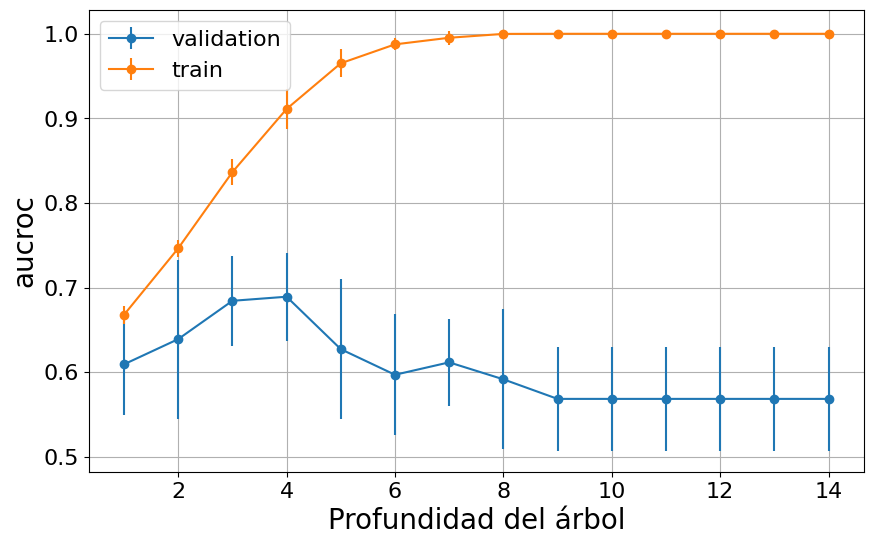
\includegraphics[width=0.4955\textwidth]{/files/src/.media/decisionTreeComplexity.png}
    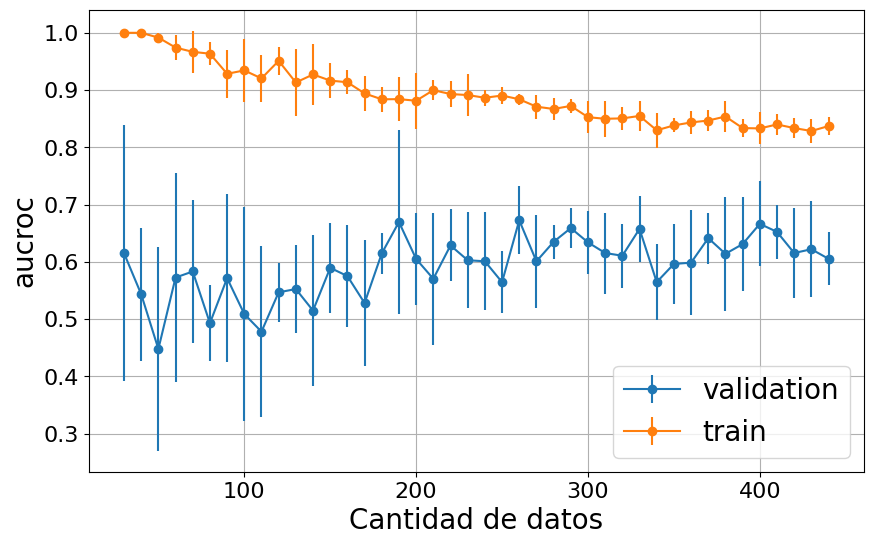
\includegraphics[width=0.4955\textwidth]{/files/src/.media/decisionTreeLearning.png}
    \caption{Clasificador \textit{decision tree}. Izquierda: Curvas de complejidad mostrando la variación del \textit{aucroc} a medida que aumenta la \textit{profundidad máxima}. Derecha: Curvas de aprendizaje mostrando la variación del \textit{aucroc} a medida que aumenta el tamaño del dataset.}
    \label{decisionTreeComplexity}
\end{figure}

Respecto a la varianza, podemos intuir que el rendimiento de este modelo va a cambiar considerablemente según el dataset utilizado en entrenamiento. Esto puede apreciarse en las barras de error\footnote{Estas corresponden a la desviación estándar de las mediciones de \textit{aucroc} para cada fold de validación.} presentes en la curva, donde en algunos casos, como para \textit{altura máxima} = 2 y 5, resultó en una diferencia de performance de más de un $10\%$ entre splits de validación. A su vez, puede verse cómo se van separando ambas curvas a medida que aumenta la \textit{profundidad máxima}. Es decir, la performance del modelo en entrenamiento aumenta mientras que en validación decrece. Esto muestra que la varianza del clasificador crece junto al hiperparámetro. El modelo parece acoplarse cada vez más al dataset.

Por otro lado, todos los resultados del algoritmo en validación se encuentran con un \textit{aucroc} por debajo de $0.75$, y con una media aproximadamente de $0.6$. En consecuencia, el modelo parecería tener poca capacidad predictiva. Sin importar el valor del hiperparámetro, es incapaz de acercarse a la distribución subyacente de los datos.

% 2. Graficar curvas de aprendizaje para cada modelo. En base a estas curvas, sacar conclusiones sobre si los algoritmos parecen haber alcanzado su límite, o bien si aumentar la cantidad de datos debería ayudar.

Por el lado de la curva de aprendizaje, podemos observar que, con pocos datos (menos de $150$ instancias), el modelo parece funcionar igual, a veces hasta peor, que un clasificador aleatorio, ya que su valor de \textit{aucroc} ronda el $0.5$ para validación. Al aumentar la cantidad de datos, ambas curvas se acercan entre sí, para luego estabilizarse en los valores de $0.85$ para el set de entrenamiento y $0.6$ para el de validación, lo que da cuenta de un sesgo moderado. Esto indicaría que el algoritmo, sin importar cuánto aumentemos el tamaño del set de entrenamiento, habría encontrado su límite de aprendizaje. 

\subsection{Linear discriminant analysis}
A partir de la configuración obtenida en la Figura \ref{lda}, generamos la curva de aprendizaje presentada en la Figura \ref{LDALearning}. En este caso, no vamos a considerar curvas de complejidad, ya que el algoritmo no cuenta con ningún hiperparámetro que, para nosotros, sirva como proxy para esta medida.

\vspace{0.5em}
\begin{figure}[!htbp]
    \centering
    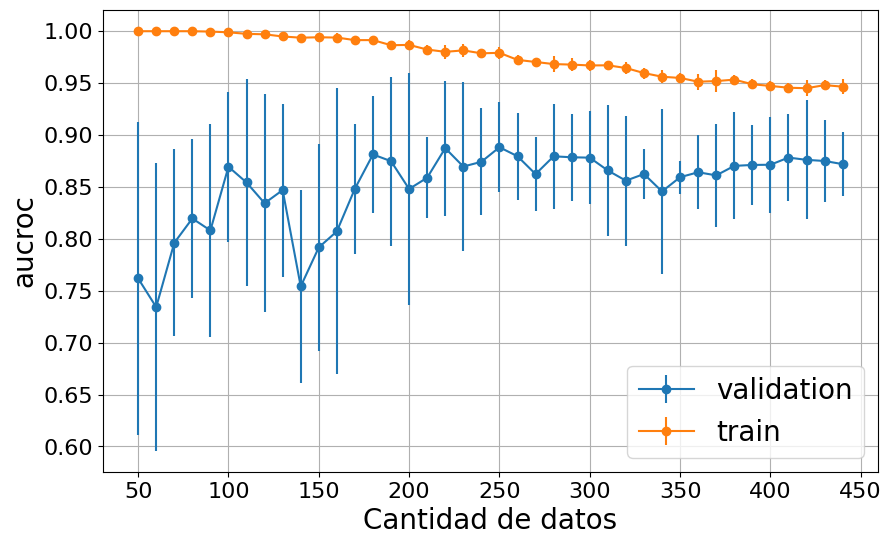
\includegraphics[width=0.49\textwidth]{/files/src/.media/LDALearning.png}
    \caption{Clasificador \textit{Linear Discriminant Analisis}. Curvas de aprendizaje mostrando la variación del \textit{aucroc} en datos de entrenamiento y validación a medida que aumenta la cantidad de datos\protect\footnotemark.}
    \label{LDALearning}
\end{figure}
\footnotetext{Dado que durante la construcción de las curvas de aprendizaje aumenta la cantidad de datos de entrenamiento, no nos pareció correcto resetear el \textit{random\_state} en el proceso de $5$-fold cross validation estratificado que produce cada medición. Luego, los resultados pueden diferir un poco con respecto a los obtenidos durante la búsqueda aleatoria.}

Podemos apreciar que el modelo posee un sesgo bajo, teniendo en cuenta que su performance se estabiliza cerca del valor $0.87$ para validación, al contar con más de $200$ datos, y de $0.95$ para entrenamiento. Esto refleja que el modelo deja de aprender y, en consecuencia, contar con más datos no debería beneficiarlo significativamente. Como detalle interesante, notamos que el mejor valor de \textit{aucroc} luego de estabilizarse fue de $0.88$ para $250$ datos.

Por último, también se puede apreciar que al aumentar la cantidad de datos, la desviación estándar se achica, lo que parece indicar que la varianza del modelo diminuye. En general, el mismo parece poseer baja varianza desde los $200$ datos, en donde la curva se estabiliza. De manera tentativa, calculamos el promedio de las deviaciones estándar a partir de este tamaño de dataset, y su valor fue de aproximadamente $0.05$.


\subsection{Support vector machines}
Basándonos en la mejor configuración de hiperparámetros hallada (ver la Figura \ref{svm}), procedimos a realizar las curva de complejidad y aprendizaje presentadas en la Figura \ref{SVMCurves}.  La curva de complejidad utiliza el hiperparámetro $C$ como proxy. El mismo permite controlar la penalización por errores de clasificación. % Un valor mayor de C significa que el modelo penalizará más los errores de clasificación lo cual implica que buscará un hiperplano de separación que clasifique correctamente la mayor cantidad posible de ejemplos de entrenamiento. Por otro lado, un valor de C menor permite que el modelo tolere más errores de clasificación y puede resultar en un hiperplano de separación más general, incluso si esto significa clasificar incorrectamente algunos ejemplos de entrenamiento.

\begin{figure}[!htbp] 
    \centering
    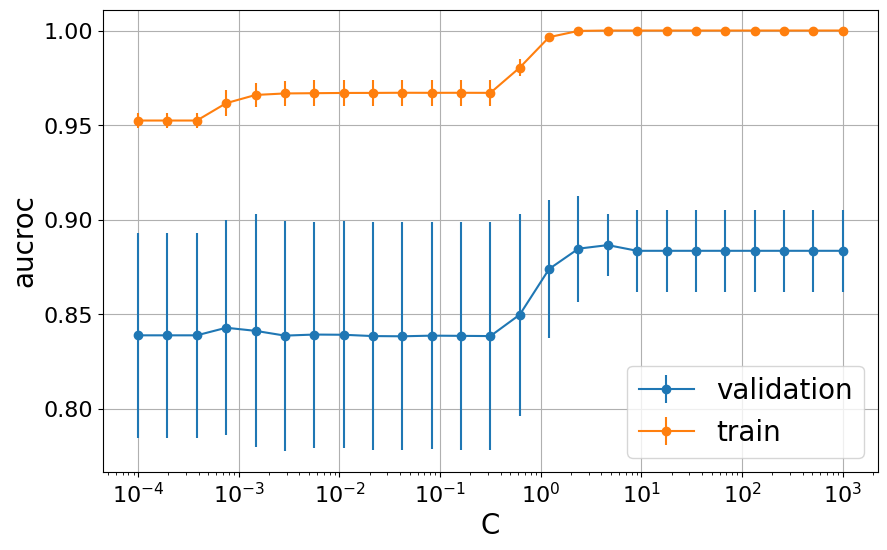
\includegraphics[width=0.49\textwidth]{/files/src/.media/SVMComplexity.png}
    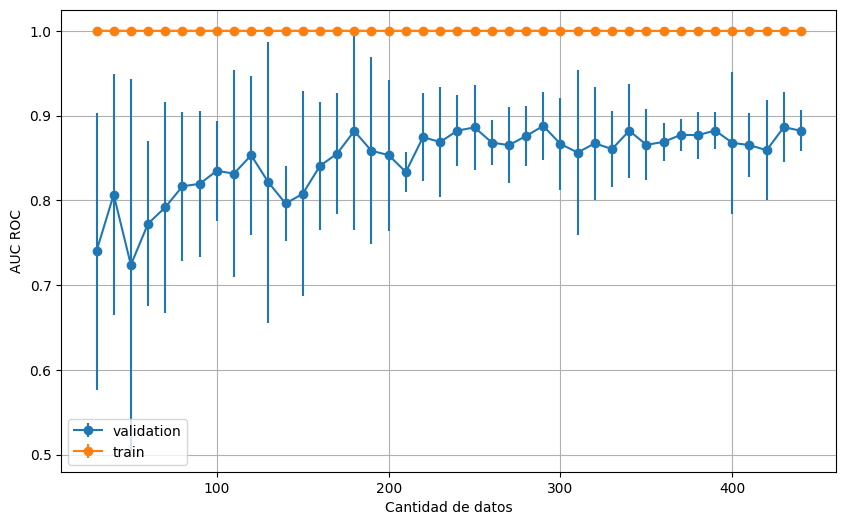
\includegraphics[width=0.49\textwidth]{/files/src/.media/SVMLearning.png}
    \caption{Clasificador \textit{SVM}. Izquierda: Curvas de complejidad mostrando la variación del \textit{aucroc} a medida que aumenta \textit{C}. Derecha: Curvas de aprendizaje mostrando la variación de la medida respecto al tamaño del dataset.}
    \label{SVMCurves}
\end{figure}

Como se puede ver en la Figura \ref{SVMCurves}, el hiperparámetro $C$ afecta a la performance del algoritmo, aunque no de forma considerable. El mismo parece ser bastante bueno para modelar el problema, ya que sin importar el valor elegido para este parámetro, el \textit{aucroc} promedio es alto. De todas maneras, una elección incorrecta de $C$ parece causar una varianza alta dentro de los folds durante la validación cruzada, por lo que parece tener un mayor impacto en la estabilidad del modelo que en la performance.
 
Por su parte, la curva de aprendizaje en la Figura \ref{svm} nos permite determinar que la cantidad de datos es suficiente para armar un modelo decente, ya que a partir de los $250$ datos, pareciera mantener una performance constante. Algo a destacar es que, a diferencia de \textit{árboles de decisión}, la desviación estándar, incluso al considerar casi todos los datos, sigue mostrando una gran variabilidad, lo cual denota una posible inestabilidad del algoritmo. 

A partir de esta cantidad, se asienta un sesgo mediano, visible en la diferencia entre la curva de aprendizaje de entrenamiento y aquella de validación. El hecho que esta primer curva nunca baje de un valor de $1$ da indicios de una posible tendencia del modelo a sobreajustar. 

\subsection{Random forests} Como última instancia de análisis, vamos a explorar el comportamiento de un modelo sustentado en técnicas de \textit{bagging}. Las mismas garantizan mayor robustez respecto a la varianza, a cuestas de un mayor costo computacional en el entrenamiento. 

Al igual que en la Sección \ref{algoritmos}, realizamos un búsqueda aleatoria para encontrar configuraciones decentes. Consideramos los siguientes hiperparámetros y rangos:

\begin{itemize}
    \item El criterio de corte: permitimos todos los criterios implementados por el algoritmo. Estos son \textit{Gini}, \textit{Entropy} y \textit{Log loss}. 
    \item La profundidad máxima: permitimos que varíe en el rango $[1,\ 4]$ de manera uniforme, dado que este rango obtuvo buenos resultados para \textit{árboles de decisión} y conlleva un menor costo computacional en el entrenamiento.
    \item La cantidad de atributos máxima a considerar por corte: permitimos que varíe de manera uniforme sobre $[1, p]$.
\end{itemize}

La Figura \ref{random_forest} muestra los mejores hiperparámetros obtenidos. Con esta configuración, procedimos a construir las curvas de complejidad ---variando la cantidad máxima de atributos--- y de aprendizaje presentadas en la Figura \ref{RF}.

\vspace{0.5em}
\begin{figure}[!htbp]
    \begin{center}
        \begin{tabular}{ |c|c|c|c| } 
         \hline
        Altura Máxima   & Criterio de corte & Atributos Máximos  & aucroc (validación) \\
        \hline
        $2$	            & \textit{Log loss} & $33$	            & $0.8117$\\
        \hline	 
        \end{tabular}
    \end{center}
    \caption{mejor resultado para la búsqueda aleatoria de hiperparámetros en el caso de \textit{random forests}.} \label{random_forest}
\end{figure}

\vspace{0.5em}
\begin{figure}[!htbp]
    \centering
    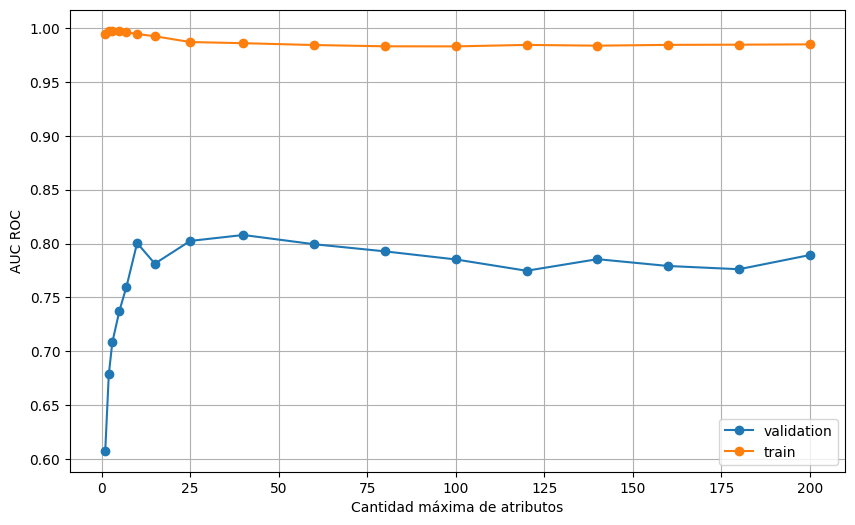
\includegraphics[width=0.49\textwidth]{/files/src/.media/randomForestComplejidad.png}
    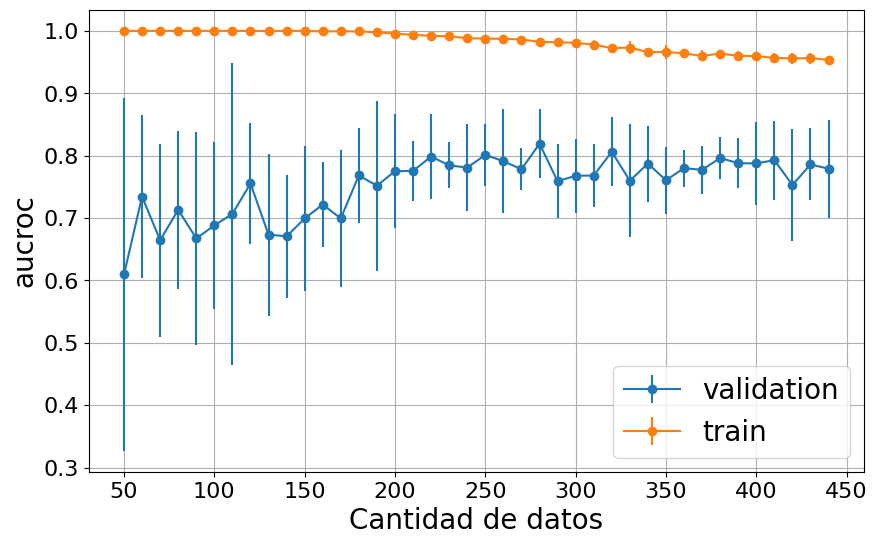
\includegraphics[width=0.49\textwidth]{/files/src/.media/randomForestAprendizaje.png}
    \caption{Clasificador \textit{Random forests}. Izquierda: Curvas de complejidad mostrando la variación del \textit{aucroc} a medida que aumenta la cantidad máxima de atributos. Derecha: Curvas de aprendizaje mostrando la variación del \textit{aucroc} a medida que aumenta el tamaño del dataset.}
    \label{RF}
\end{figure}

Respecto a la curva de complejidad, observamos ---no sorprendentemente--- que un valor bajo en la cantidad máxima de atributos permitidos genera un impacto negativo en la performance del algoritmo. Esto tiene sentido, ya que éste hiperparámetro guía cuántos atributos cada árbol de decisión va a poder utilizar al evaluar cortes. Está claro que, a menor cantidad de atributos a considerar, menor la posibilidad de encontrar un buen corte.

Sin embargo, la curva nos muestra otro resultado que es menos intuitivo: la cantidad máxima de atributos permitidos rápidamente alcanza su límite repecto a su capacidad de impactar en la performance del modelo. Luego, a medida que sigue aumentando, incluso parece disminuir ligeramente. Esto es particularmente atractivo, ya que, si bien a medida que crece la performance no mejora considerablemente, sí afecta directamente en el costo computacional. Una posible explicación para este fenómeno es que mientras más atributos se consideren en cada corte, menos variabilidad vamos a encontrar entre los árboles que componen al bosque. Es decir, los árboles resultantes van a ser más parecidos entre sí, por lo que no van a poder complementarse mutuamente.  

Por un lado, vimos en la búsqueda aleatoria que un valor de $33$ arrojó los mejores resultados. Consideramos que tendría sentido usar un valor como $\log(p)$ o $\sqrt{p}$ para lograr un buen \textit{trade-off} entre performance y complejidad computacional, manteniendo la dependencia respecto a la cantidad de atributos.   

Por otro lado, la curva de aprendizaje de la Figura \ref{RF} muestra que a partir de $200$ datos la performance del modelo parece estabilizarse, sin poder discernir niguna tendencia alcista. Concluimos que la cantidad de datos provista es suficiente para generar un modelo decente basado en \textit{random forests}. 

Algo interesante a destacar es que la desviación estándar se vuelve chica para modelos entrenados con suficientes datos, lo que implica una menor varianza del modelo. A su vez, la brecha entre las curvas de entrenamiento y validación en el gráfico de aprendizaje da cuenta de un leve sesgo del modelo.
